\section{Питание}

Важнейшей составляющей радиосредства являются фидеры между радиопередатчиком и передающей антенной или между приемной антенной и радиоприемником. Фидеры радиосредств, используемых для целей связи и вещания, можно разделить на два обособленных класса: открытые и закрытые. Открытые фидеры — это, как правило, двухпроводные или четырехпроводные симметричные линии передачи. Закрытые фидеры представляют собой коаксиальный кабель или полый металлический волновод. Открытые линии применяются на частотах до 30 МГц, кабельные — до 3000 МГц, волноводные — до 30 ГГц.

\begin{figure}[H]
    \centering
    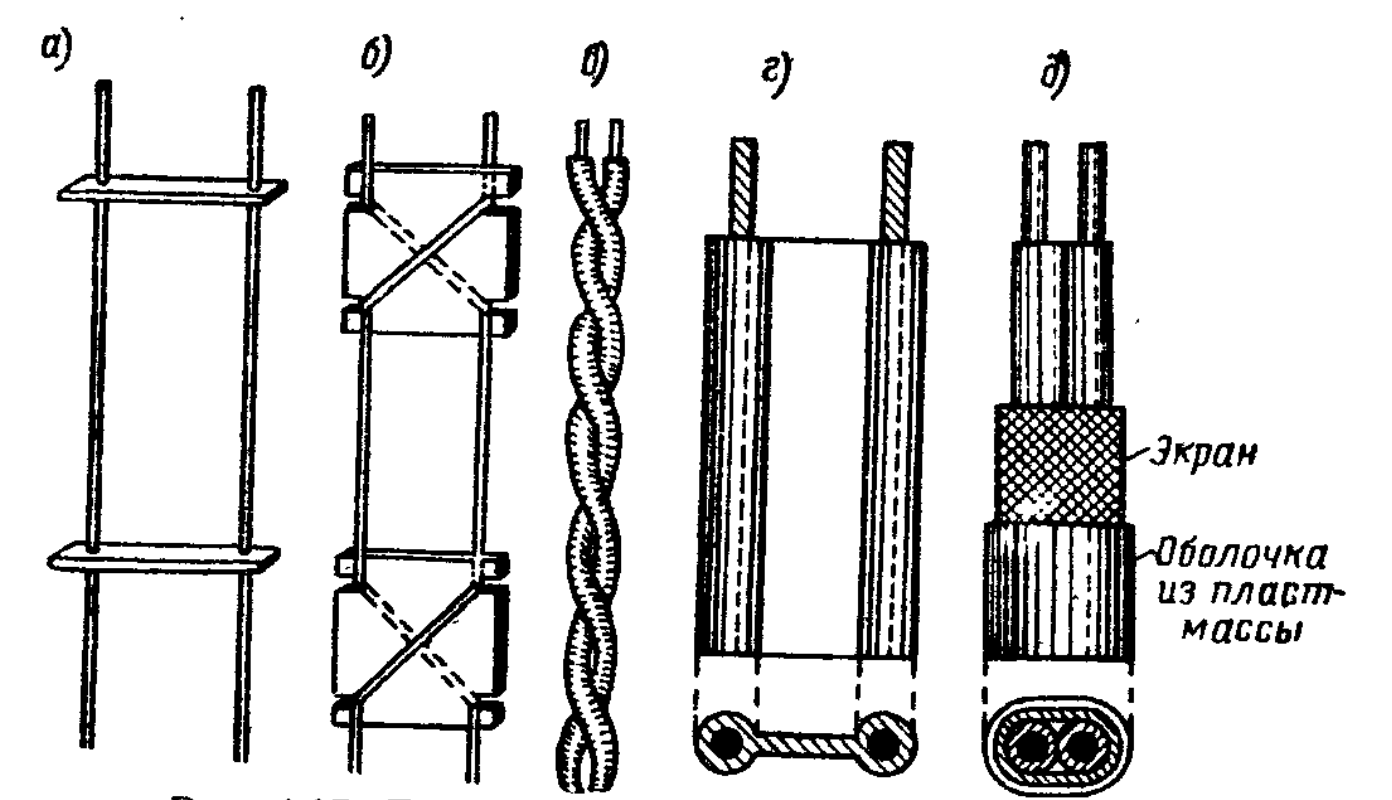
\includegraphics[width=.9\textwidth]{img/fider_types.png}
    \caption{Типы симметричных фидерных линий}
    \label{fig:fider_types}
\end{figure}

Несколько типичных конструкций cимметричных фидеров показаны на рис. \ref{fig:fider_types} Для фидеров по рис.\ref{fig:fider_types} а и б, изолирующие распорки делают из высококачественного диэлектрика. Фидер с перекрещивающимися проводами (рис.\ref{fig:fider_types} б) применяется для приемных антенн. Он обладает меньшим антенным эффектом. В простейшем случае для приемных антенн используется фидер, рис.\ref{fig:fider_types} в, состоящий из двух свитых вместе изолированных проводов (в виде шнура). Очень удобны симметричные кабели ленточного типа (рис.\ref{fig:fider_types} г), имеющие два провода, запрессованные в ленту из гибкой пластмассы.

Для уменьшения емкости лента между проводами делается тонкой или имеет отверстия. На рис.\ref{fig:fider_types} д, показан симметричный экранированный кабель, у которого антенный эффект отсутствует. Симметричные кабели, выпускаемые промышленностью, обычно имеют $Z$ от 30 до 300 ом.

Как видно, некоторые типы симметричных фидеров могут быть изготовлены самостоятельно из двух проводов (рис.\ref{fig:fider_types} а, б и в).Применяемые для несимметричных фидеров коаксиальные кабели изготовляются исключительно в заводских условиях. Промышленность выпускает много различных типов коаксиальных высокочастотных кабелей. Большинство из них имеет волновое сопротивление от 50 до 90 ом и рассчитано на пробивное напряжение от 1 до 15 кв. Устройство наиболее распространенного кабеля со сплошной изоляцией показано на рис.\ref{fig:koax}. 

\begin{figure}[H]
    \centering
    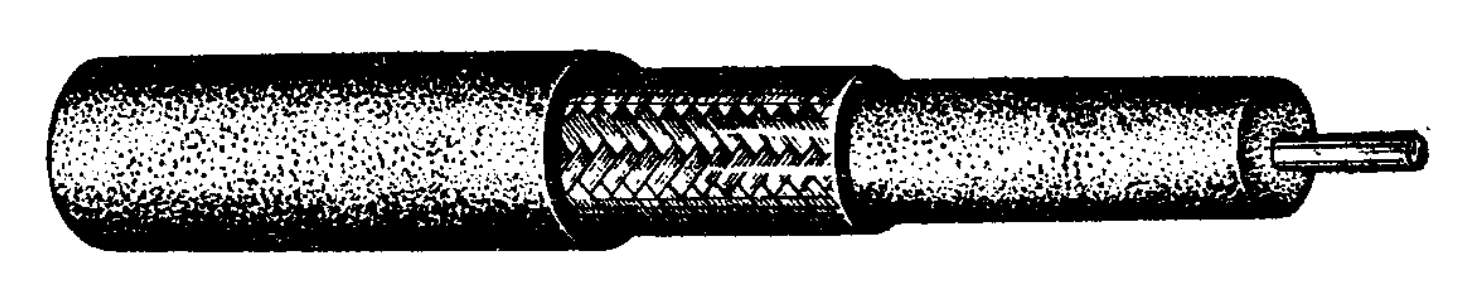
\includegraphics[width=.9\textwidth]{img/koax.png}
    \caption{Коаксиальный кабель для фидерной линии}
    \label{fig:koax}
\end{figure}

В таких кабелях в качестве изоляции применяется гибкая пластмасса, вносящая малые потери на высоких частотах (например, полиэтилен). Внутренний провод бывает одножильный или многожильный. Внешний провод сделан в виде оплетки из медных проволочек и покрыт сверху защитной пластмассовой оболочкой.

Основным требованием, предъявляемым к фидерам, является доведение до минимума потерь энергии в нем. В зависимости от конструкции фидера потери энергии могут определяться: нагреванием металлических элементов, изоляторов и окружающей среды, а также излучением (в случае открытого фидера). Качество фидера, в смысле потерь энергии, определяется коэффициентом полезного действия. 

\textbf{Коэффициентом полезного действия} фидера передающей антенны называется отношение мощностей радиочастотного сигнала на его выходе и входе.



К коэффициенту полезного действия фидеров приемных антенн до 30 МГц (диапазоны НЧ, СЧ и ВЧ) обычно не предъявляются такие жесткие требований, как к этому же параметру фидеров передающих антенн. В этих диапазонах интенсивность внешних помех велика. При прохождении через фидер с потерями внешние помехи претерпевают такое же ослабление, как и полезный сигнал. Поэтому отношение мощностей сигнала и внешних помех на входе и на выходе фидера сохраняется. На более высоких частотах (диапазоны ОВЧ, УВЧ и СВЧ), когда мощность внутренних шумов приемных устройств соизмерима или превосходит мощность внешних помех, значение коэффициента полезного действия фидера необходимо по возможности увеличивать. Фидер должен обладать достаточной электрической прочностью, т.е. должен быть рассчитан на передачу требуемой мощности без опасности электрического пробоя. В фидере, как и в передающей антенне, может образоваться факельное истечение. В худшем случае отдельные провода могут расплавиться и сделать фидер неработоспособным.



Фидеры должны быть свободны от антенного эффекта, т.е. сами по себе не должны излучать или принимать электромагнитные волны. Передающая антенна почти всегда находится не в свободном пространстве. В непосредственной близости от неё могут оказаться многие объекты. Один из ближайших и принципиально не удаляемых предметов окружения антенны является её фидер. Ближнее поле излучения антенны может нарушить симметрию противофазных токов в фидере, и он начнет излучать электромагнитные волны. Антенный эффект абсолютно нежелателен из-за возрастания потерь в фидере (потерь на излучение) и вследствие искажения диаграммы направленности передающей антенны.

Последствия антенного эффекта в фидере приемной антенны могут оказаться ещё более неприятными, поскольку они могут свести на нет все достоинства направленной антенны и дать резкое увеличение мощности внешних помех на входе радиоприемника.

Фидеры характеризуются рабочей полосой частот. В пределах диапазона частот параметры фидера не должны выходить за пределы допусков, установленных техническими требованиями. Критичным параметром может оказаться, например коэффициент полезного действия, фидера. Его низкое значение является прямым следствием рассогласования фидера с антенной.

Важным параметром фидера является его волновое сопротивление, которое определяется конфигурацией, геометрическими размерами и материалом, заполняющим пространство меду проводами. Значение волнового сопротивления фидера приобретает исключительную роль в решении вопросов согласования фидера с передающей антенной и передатчиком или с приемной антенной и приемником.

Открытые фидеры строятся непосредственно на радиотехническом объекте с использованием документации типовых проектов, в которые закладываются решения, обеспечивающие достижение требуемых параметров и характеристик фидера. Закрытые фидеры изготавливаются на специализированных предприятиях. Их параметры и характеристики обычно гарантируются и указываются в сертификате на фидер.
